\documentclass[12pt, a4paper]{article}

\usepackage[utf8]{inputenc}

% Limit the page margin to only 1 inch.
\usepackage[margin=1in]{geometry}

%Imports biblatex package
\usepackage[
backend=biber,
style=alphabetic
]{biblatex}
\addbibresource{../math-342w.bib}

% Enables the `align' environment.
\usepackage{amsmath}

% Provides useful environments, such as:
% - \begin{proof} ...\end{proof}
\usepackage{amsthm}
\newtheorem{proposition}{Proposition}
\theoremstyle{definition}
\newtheorem*{definition}{Definition}
\newtheorem{theorem}{Theorem}
\newtheorem{corollary}{Corollary}

% Enables using \mathbb{}, for example \mathbb{N} for the set of natural numbers.
\usepackage{amssymb}

% Allows using letters in enumerate list environment. Use, for example:
%\begin{enumerate}[label=(\alph*)]
% ...
%\end{enumerate}
\usepackage[inline]{enumitem}

% Enable importing external graphic files and provides useful commands, like \graphicspath{}
\usepackage{graphicx}
% Images are located in a directory called "images" in the current directory.
\graphicspath{{./images/}}

% Make links look better by default.
% See: https://tex.stackexchange.com/questions/823/remove-ugly-borders-around-clickable-cross-references-and-hyperlinks
\usepackage[hidelinks]{hyperref}
\usepackage{xcolor}
\hypersetup{
	colorlinks,
	linkcolor={red!50!black},
	citecolor={blue!50!black},
	urlcolor={blue!80!black}
}

% Code Listings. Source:
% https://stackoverflow.com/questions/3175105/inserting-code-in-this-latex-document-with-indentation
\usepackage{listings}
\usepackage{color}
\usepackage[most]{tcolorbox}

\definecolor{dkgreen}{rgb}{0,0.6,0}
\definecolor{gray}{rgb}{0.5,0.5,0.5}
\definecolor{mauve}{rgb}{0.58,0,0.82}

\lstset{frame=tb,
	language=Java,
	aboveskip=3mm,
	belowskip=3mm,
	showstringspaces=false,
	columns=flexible,
	basicstyle={\small\ttfamily},
	numbers=none,
	numberstyle=\tiny\color{gray},
	keywordstyle=\color{blue},
	commentstyle=\color{dkgreen},
	stringstyle=\color{mauve},
	breaklines=true,
	breakatwhitespace=true,
	tabsize=3
}

\newcommand{\prob}{\text{P}}
%\newcommand{\complement}{\mathsf{c}}
\title{Lecture 10: MATH 342W: Introduction to Data Science and Machine Learning}
\author{Sergio E. Garcia Tapia\thanks{Based on lectures of Dr. Adam Kapelner at Queens College.
See also the \href{https://github.com/kapelner/QC_MATH_342W_Spring_2025}{course GitHub page}.}}
\date{March 4, 2025 (last updated \today)}

\begin{document}
	\maketitle
	\section*{Uniqueness of Orthogonal Projection Matrix}
	Let $X$ be a matrix of dimension $n\times (p+1)$ (where $n > p+1$) and full rank.
	Then $\text{rank}(X)=p+1$. Let $X_\perp$ be a matrix of dimension $n\times (n-[p+1])$,
	where the columns $X_\perp$ are a basis of $co\ell[X]^\perp$ (the orthogonal complement
	of the column space of $X$). Then $\text{rank}(X_\perp)=n-(p+1)$.
	
	Let $H$ be an orthogonal projection matrix onto the column space of $X$. Since each
	column of $X$ is already in the column space of $X$, we know (and indeed we have shown
	before) that
	\begin{align*}
		HX=X
	\end{align*}
	On the other hand, since every column of $X_\perp$ is in the orthogonal complement
	of $co\ell [X]$, projecting the column with $H$ yields $\textbf{0}_n$ for each column:
	\begin{align*}
		HX_\perp = \mathbf{0}_{n\times (n-[p+1])}
	\end{align*}
	Let $X_{\text{full}}=[X \mid X_\perp]$, meaning $X_{\text{full}}$ is the matrix obtained
	by concatenating the columns of $X$ and columns of $X_\perp$ into an $n\times n$ matrix.
	Since $X$ and $X_{\perp}$ are each full rank, and since columns of $X$ and those of $X_\perp$
	are orthogonal, it follows that all columns combined make up a basis of $\mathbb{R}^n$.
	Thus, $X_{\text{full}}$ an $n\times n$ matrix of full rank and hence invertible.
	We will use this fact to show that the orthogonal projection matrix $H$ is unique.
	\begin{tcolorbox}[breakable]
		\begin{theorem}
			\label{thm:ortho-proj-mat-unique}
			Let $X$ be a matrix of dimension $n\times (p+1)$ that is full rank. Then
			the orthogonal projection matrix onto the column space of $X$ is unique.
		\end{theorem}
		\begin{proof}
			We have already shown that an orthogonal projection matrix exists,
			given by $H=X(X^\top X)^{-1}X^\top$. Suppose $H'$ is also an orthogonal
			projection matrix onto the column space of $X$. Let $X_{\perp}$ be the
			matrix whose columns contain a basis of the $co\ell[X]^\perp$.
			Then the matrix $X_{\text{full}}=[X\mid X_\perp]$ is full rank.
			Since $H$ and $H'$ are both orthogonal projection matrices onto
			$co\ell[X]$, we have
			\begin{align*}
				H'X_{\text{full}}=[X \mid \mathbf{0}_{n\times (n-[p+1])}]=HX_\text{full}
			\end{align*}
			Since $X_{\text{full}}$ is full rank, it is invertible, so
			\begin{align*}
				H'X_{\text{full}} &= HX_{\text{full}}\\
				(H'X_{\text{full}})X_{\text{full}}^{-1} &= (HX_{\text{full}})X_{\text{full}}^{-1}\\
				H'(X_{\text{full}}X_{\text{full}}^{-1}) &= H(X_{\text{full}}X_{\text{full}}^{-1})\\
				H'I_{n} &= H I_n
				\tag{$I_n$ is the identity matrix}\\
				H'&=H
			\end{align*}
		\end{proof}
	\end{tcolorbox}
	\section*{Sum of Projections}
	Let $\mathbf{a}\in \mathbb{R}^n$, and let $\mathbf{v}_1$ and $\mathbf{v}_2$ be
	two linearly independent vectors in $\mathbb{R}^n$. Let $V=[\mathbf{v}_1 \mid \mathbf{v}_2]$,
	meaning $V$ is an $n\times 2$ matrix whose columns are $\mathbf{v}_1$ and $\mathbf{v}_2$.
	Is the following statement true?
	\begin{align}
		\underset{co\ell [V]}{\text{proj}(\mathbf{a})}
		\stackrel{?}{=}\underset{\text{span}(\mathbf{v}_1) }{\text{proj}(\mathbf{a})}
		+\underset{\text{span}(\mathbf{v}_2) }{\text{proj}(\mathbf{a})}
		\label{eqn:sum-of-projections-conjecture}
	\end{align}
	Recall that if $\mathbf{u}$ is a vector, then
	\begin{align*}
		\underset{\text{span}(\mathbf{u} }{\text{proj}(\mathbf{a})} =
		\mathbf{u}(\mathbf{u}^\top \mathbf{u})^{-1}\mathbf{u}^\top \mathbf{a}
		=\frac{\mathbf{u}\mathbf{u}^\top}{\|\mathbf{u}\|^2} = H_{\mathbf{u}}\mathbf{a}
	\end{align*}
	Hence, if $H_1$ is the orthogonal projection matrix onto $\text{span}(\mathbf{v}_1)$,
	$H_2$ is the orthogonal projection matrix onto $\text{span}(\mathbf{v}_1)$, and
	$H$ is the orthogonal projection matrix onto $co\ell[V]$, then
	Equation~\ref{eqn:sum-of-projections-conjecture} is equivalent to
	\begin{align*}
		H\mathbf{a} \stackrel{?}{=} H_1\mathbf{a} + H_2\mathbf{a}=(H_1+H_2)\mathbf{a}
	\end{align*}
	Now, is $H_1+H_2$ an orthogonal projection matrix? If so, then the uniqueness
	implied by Theorem~\ref{thm:ortho-proj-mat-unique} would imply $H=H_1+H_2$.
	Recall that $P$ is a projection matrix if $(\mathbf{v}-P\mathbf{v})^\top(P\mathbf{w})=0$
	for all $\mathbf{v},\mathbf{w}\in\mathbb{R}^n$. Here we let $P=H_1+H_2$ and
	$\mathbf{v}=\mathbf{w}=\mathbf{a}$:
	\begin{align*}
		H_1+H_2\text{ is an orthogonal projection }
		\iff ( (H_1+H_2)\mathbf{a} )^\top(\mathbf{a} - (H_1+H_2)\mathbf{a})=0
	\end{align*}
	In light of this equivalence, we will explore what it takes to make it true.
	\begin{align}
		0 &\stackrel{?}{=}( (H_1+H_2)\mathbf{a} )^\top(\mathbf{a} - (H_1+H_2)\mathbf{a})
		\tag{Unverified conjecture}\nonumber\\
		  &=( H_1\mathbf{a} + H_2\mathbf{a} )^\top(\mathbf{a} - (H_1\mathbf{a} + H_2\mathbf{a}))
		  \tag{Linearity}\nonumber\\
		  &=(H_1\textbf{a}+H_2\mathbf{a})^\top \mathbf{a} -
		  (H_1\textbf{a}+H_2\mathbf{a})^\top (H_1\mathbf{a} + H_2\mathbf{a})
		  \tag{Distributivity}\nonumber\\
		  &=((H_1\textbf{a})^\top+(H_2\textbf{a})^\top) \mathbf{a} -
		  ((H_1\textbf{a})^\top+(H_2\mathbf{a})^\top) (H_1\mathbf{a} + H_2\mathbf{a})
		  \tag{$(A+B)^\top=A^\top+B^\top$}\nonumber\\
		  &=(H_1\mathbf{a})^\top \mathbf{a} + (H_2\mathbf{a})^\top\mathbf{a}
		  -( (H_1\mathbf{a})^\top H_1\mathbf{a} + (H_1\mathbf{a})^\top H_2\mathbf{a}
		    + (H_2\mathbf{a})^\top H_1\mathbf{a} + (H_2\mathbf{a})^\top H_2\mathbf{a} )\nonumber\\
		  &=\mathbf{a}^\top H_1^\top\mathbf{a}  + \mathbf{a}^\top H_2^\top\mathbf{a}
		  -\mathbf{a}^\top H_1^\top H_1\mathbf{a} - \mathbf{a}^\top H_1^\top H_2\mathbf{a}
		  -\mathbf{a}^\top H_2^\top H_1\mathbf{a} - \mathbf{a}^\top H_2^\top H_2\mathbf{a}
		  \nonumber\\
		  &=\mathbf{a}^\top \underbrace{(H_1^\top -H_1^\top H_1)}_{0}\mathbf{a}
		  +\mathbf{a}^\top\underbrace{(H_2^\top -H_2^\top H_2)}_{0}\mathbf{a}
		  -\mathbf{a}^\top H_1^\top H_2\mathbf{a}
		  -\mathbf{a}^\top H_2^\top H_1\mathbf{a}\nonumber\\
		  &=-(H_1\mathbf{a})^\top H_2\mathbf{a} -(H_2\mathbf{a})^\top H_1\mathbf{a}
		  \tag{$H_1$ and $H_2$ are idempotent and symmetric}\\
		  &=-(H_1\mathbf{a})\cdot (H_2\mathbf{a}) - (H_2\mathbf{a})\cdot (H_1\mathbf{a})
		  \tag{Definition of dot product}\\
		  &=-2(H_1\mathbf{a})\cdot (H_2\mathbf{a})
		  \tag{Dot product is commutative}
	\end{align}
	The last equality is zero if and only if the dot product is zero.
	Now recall that $\mathbf{a}$ is arbitrary, that $H_1\mathbf{a}$ projects $\mathbf{a}$
	onto the one-dimensional subspace $\text{span}(\mathbf{v}_1)$, and $H_2\mathbf{a}$ projects
	$\mathbf{a}$ onto the one-dimensional subspace $\text{span}(\mathbf{v}_2)$. Thus
	there exists $c_1,c_2\in\mathbb{R}$ such that $H_1\mathbf{a}=c_1\mathbf{v}_1$ and
	$H_2\mathbf{a}=c_2\mathbf{v}_2$, so we may write
	\begin{align*}
		(H_1\mathbf{a})\cdot (H_2\mathbf{a}) &= (c_1\mathbf{v}_1)\cdot(c_2\mathbf{v}_2)\\
		&=c_1c_2(\mathbf{v}_1\cdot\mathbf{v}_2)\\
		&=c_1c_2(\|\mathbf{v}_1\| \|\mathbf{v}_2\|\cos\theta)
	\end{align*}
	The last equality is a consequence of the Schwarz inequality (see \cite{axler}), and
	$\theta$ represents the angle between $\mathbf{v}_1$ and $\mathbf{v}_2$.
	In order for this to hold for all $\mathbf{a}$, we require $\cos\theta=0$,
	and hence $\theta=90^\circ$. We have verified the following fact.
	\begin{tcolorbox}[breakable]
		\begin{theorem}
			\label{thm:sum-of-orth-projs}
			Let $\mathbf{v}_1$ and $\mathbf{v}_2$ be two linearly independent vectors
			in $\mathbb{R}^n$. Let $V=\text{span}(\mathbf{v}_1, \mathbf{v}_2)$,
			$V_1=\text{span}(\mathbf{v}_1)$, and $V_2=\text{span}(\mathbf{v}_2)$.
			Then, for all $\mathbf{a}\in\mathbb{R}^n$,
			\begin{align*}
				\text{proj}_V(\mathbf{a}) =
				\text{proj}_{V_1}(\mathbf{a}) + \text{proj}_{V_2}(\mathbf{a})
			\end{align*}
			if and only if $\mathbf{v}_1$ and $\mathbf{v}_2$ are orthogonal.
		\end{theorem}
	\end{tcolorbox}
	\begin{tcolorbox}[breakable]
		\begin{corollary}
			\label{corollary:sum-ortho-projs}
			Let $\mathbf{v}_1, \mathbf{v}_2\ldots,\mathbf{v}_d$ be a linearly independent list of vectors
			in $\mathbb{R}^n$. Let $V=\text{span}(\mathbf{v}_1, \mathbf{v}_2,\ldots,\mathbf{v}_d)$,
			$V_k=\text{span}(\mathbf{v}_k)$ for all $k$ such that $1\leq k\leq d$.
			Then, for all $\mathbf{a}\in\mathbb{R}^n$,
			\begin{align*}
				\text{proj}_V(\mathbf{a}) = \sum_{k=1}^{d}\text{proj}_{V_k}(\mathbf{a})
			\end{align*}
			if and only if the list $(\mathbf{v}_1,\mathbf{v}_2,\ldots,\mathbf{v}_d)$
			is orthogonal (meaning all vectors are pairwise orthogonal).
		\end{corollary}
	\end{tcolorbox}
	See Figure~\ref{fig:sum-of-orthogonal-projections} for a depiction of the statement
	Theorem~\ref{thm:sum-of-orth-projs}.
	\begin{figure}
		\centering
		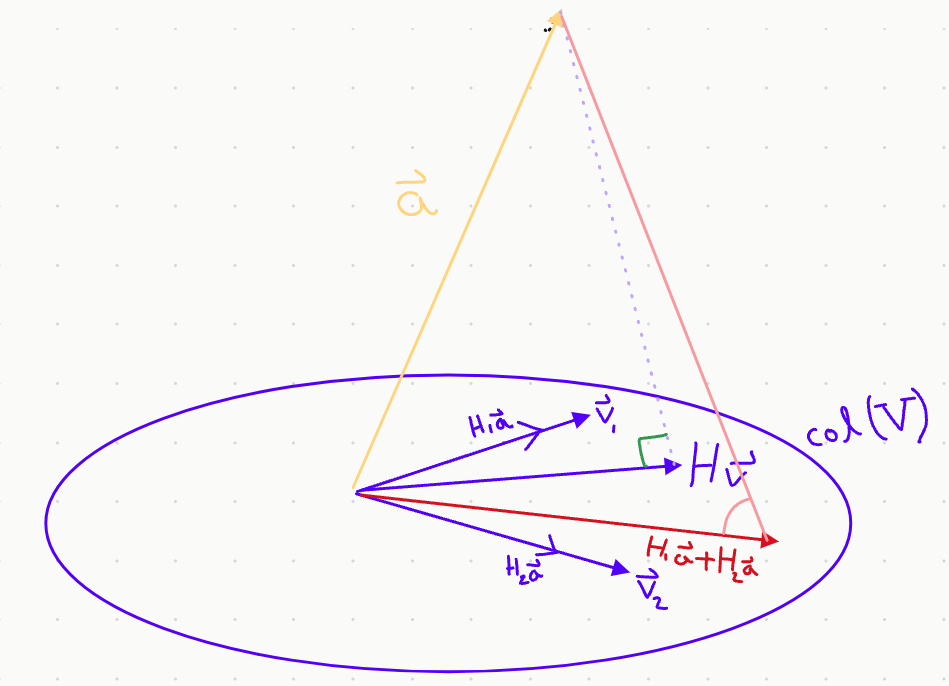
\includegraphics[width=0.8\textwidth]{sum-of-orthogonal-projections}
		\caption{Projecting $\mathbf{a}$ with $H_1$, $H_2$, and $H$.}
		\label{fig:sum-of-orthogonal-projections}
	\end{figure}
	Effectively, the theorem says that $H_1+H_2$ is not necessarily an orthogonal projection.
	\section*{Projection Matrices onto Dimension 1 Subspaces}
	Suppose $\mathbf{v}_k$ is a nonzero vector in $\mathbb{R}^n$.
	Recall from linear algebra that
	\begin{align*}
		\underset{\text{span}(\mathbf{v}_k)}{\text{proj}}(\mathbf{a})
		&:=\frac{\mathbf{v}_k^\top \mathbf{a}}{\|\mathbf{v}_k\|^2}\mathbf{v}_k
	\end{align*}
	Let's focus on the portion that says $(\mathbf{v}_k^\top \mathbf{a})\mathbf{v}_k$.
	It turns out this is equivalent to $\mathbf{v}_k\mathbf{v}_k^\top \mathbf{a}$.
	Suppose that we let $\mathbf{u}$ be their difference:
	\begin{align*}
		\mathbf{u} := (\mathbf{v}_k^\top \mathbf{a})\mathbf{v}_k - (\mathbf{v}_k\mathbf{v}_k^\top \mathbf{a})
	\end{align*}
	Now let $\mathbf{b}$ be any vector in $\mathbb{R}^n$. Multiplying by $\mathbf{b}^\top$ on the left
	we get:
	\begin{align*}
		\mathbf{b}^\top \mathbf{u}
		&= \mathbf{b}^\top(\mathbf{v}_k^\top \mathbf{a})\mathbf{v}_k -
		\mathbf{b}^\top(\mathbf{v}_k\mathbf{v}_k^\top \mathbf{a})\\
		&=(\mathbf{v}_k^\top \mathbf{a})\mathbf{b}^\top\mathbf{v}_k
		-(\mathbf{b}^\top\mathbf{v}_k)(\mathbf{v}_k^\top \mathbf{a})
		\tag{Associativity: $A(BC)=(AB)C$}\\
		&=0
	\end{align*}
	Since $\mathbf{b}$ is arbitrary, this implies $\mathbf{u}$ is orthogonal to every vector
	in $\mathbb{R}^n$, and so it must be the zero vector. Thus we have:
	\begin{align}
		\label{eqn:1d-projection}
		\underset{\text{span}(\mathbf{v}_k)}{\text{proj}}(\mathbf{a})
		&=\frac{\mathbf{v}_k^\top \mathbf{a}}{\|\mathbf{v}_k\|^2}\mathbf{v}_k
		=\frac{\mathbf{v}_k\mathbf{v}_k^\top}{\|\mathbf{v}_k\|^2}\mathbf{a}
	\end{align}
	Notice that since $\mathbf{v}_k$ is $n\times 1$, the product $\mathbf{v}_k\mathbf{v}_k^\top$
	is an $n\times n$ matrix, which in fact is of rank 1 because every row is a multiple
	of $\mathbf{v}_k^\top$.
	
	Let $\mathbf{v}_1,\mathbf{v}_2,\ldots,\mathbf{v}_d$ be a mutually orthogonal list
	of (nonzero) vectors in $\mathbb{R}^n$, meaning that $\mathbf{v}_k^\top\mathbf{v}_j=0$
	for all $1\leq k,j\leq d$ where $k\neq j$. Let
	$V=[\mathbf{v}_1 \mid \mathbf{v}_2 \mid \cdots\mid \mathbf{v}_d]$
	be an $n\times d$ matrix made by concatenating the vectors in this orthogonal list.
	Let $\mathbf{a}\in\mathbb{R}^n$. Then
	\begin{align*}
		\underset{co\ell [V]}{\text{proj}(\mathbf{a})}
		&= \sum_{k=1}^{d}\underset{\text{span}(\mathbf{v}_k)}{\text{proj}(\mathbf{a})}
		\tag{Corollary~\ref{corollary:sum-ortho-projs}}\\
		&=\sum_{k=1}^{d}\frac{\mathbf{v}_k\mathbf{v}_k^\top}{\|\mathbf{v}_k\|^2}\mathbf{a}
		\tag{Equation~\ref{eqn:1d-projection}}\\
		&=\underbrace{\left(\sum_{k=1}^{d}\frac{\mathbf{v}_k\mathbf{v}_k^\top}{\|\mathbf{v}_k\|^2}\right)}_{H}
		\mathbf{a}\\
		&=H\mathbf{a}
	\end{align*}
	Again by Corollary~\ref{corollary:sum-ortho-projs}, $H$ is an orthogonal projection
	matrix onto $co\ell[V]$. In particular, it can be expressed as a sum of $d$ orthogonal
	projection matrices, each of rank 1.
	
	Let's simplify the sum by \textit{normalizing} the vectors $\mathbf{v}_k$, which means we re-scale them
	to have length $1$. Let $\mathbf{q}_k := \frac{\mathbf{v}_k}{\|\mathbf{v}_k\|}$,
	so $\|\mathbf{q}_k\|=1$. The list $(\mathbf{q}_1,\mathbf{q}_2,\ldots,\mathbf{q}_d)$
	is still orthogonal because rescaling a vector does not change its direction,
	but since they are normalized now we refer to it as an \textit{orthonormal list}.
	If we let $Q:=[\mathbf{q}_1 \mid \mathbf{q}_2\mid \cdots |\mathbf{q}_d]$, then
	we refer to $Q$ as an \textit{orthonormal matrix}. Now we can write
	\begin{align*}
		\underset{co\ell [Q]}{\text{proj}(\mathbf{a})}
		&= \sum_{k=1}^{d}\underset{\text{span}(\mathbf{q}_k)}{\text{proj}(\mathbf{a})}
		\tag{Corollary~\ref{corollary:sum-ortho-projs}}\\
		&=\sum_{k=1}^{d}\frac{\mathbf{q}_k\mathbf{q}_k^\top}{\|\mathbf{q}_k\|^2}\mathbf{a}
		\tag{Equation~\ref{eqn:1d-projection}}\\
		&=\sum_{k=1}^{d}(\mathbf{q}_k\mathbf{q}_k^\top)\mathbf{a}
		\tag{since $\|\mathbf{q}_k\|=1$}\\
	\end{align*}
	Thus, rather than our old formula $X(X^\top X)^{-1}X^\top$ for a projection matrix, we can
	use $\sum_{k=1}^{d}\mathbf{q}_k\mathbf{q}_k^\top$, where we sum $d$ matrices each of rank 1.
	\section*{Properties of Orthonormal Matrices}
	Let $Q$ by an $n\times d$ orthonormal matrix. Then $Q^\top$ is $d\times n$.
	Recall that the columns are pairwise orthogonal, so
	\begin{align*}
		\mathbf{q}_k^\top\mathbf{q}_j = \begin{cases}
			1 & k = j\\
			0 & k \neq j
		\end{cases}
	\end{align*}
	so
	\begin{align*}
		Q^\top Q=\begin{bmatrix}
			\cdots & \mathbf{q}_1^\top & \cdots\\
			\vdots & \vdots& \vdots\\
			\cdots & \mathbf{q}_d^\top & \cdots
		\end{bmatrix}
		\begin{bmatrix}
			\vdots & \cdots & \vdots\\
			\mathbf{q}_1 & \cdots & \mathbf{q}_d\\
			\vdots & \cdots & \vdots
		\end{bmatrix}=
		I_{d\times d}
	\end{align*}
	where $I_{d\times d}$ is the identity matrix. What about $QQ^\top$? This
	is an $n\times n$ matrix:
	\begin{align*}
		QQ^\top&=\begin{bmatrix}
			\vdots & \cdots & \vdots\\
			\mathbf{q}_1 & \cdots & \mathbf{q}_d\\
			\vdots & \cdots & \vdots
		\end{bmatrix}
		\begin{bmatrix}
			\cdots & \mathbf{q}_1^\top & \cdots\\
			\vdots & \vdots& \vdots\\
			\cdots & \mathbf{q}_d^\top & \cdots
		\end{bmatrix}\\
		&=\mathbf{q}_1\mathbf{q}_1^\top+\mathbf{q}_2\mathbf{q}_2^\top+\cdots\mathbf{q}_d\mathbf{q}_d^\top\\
		&=H
	\end{align*}
	Let's verify that $QQ^\top$ is indeed an orthogonal projection matrix:
	\begin{enumerate}[label=(\roman*)]
		\item \textbf{Symmetry}:
		\begin{align*}
			(QQ^\top)^\top = (Q^\top)^\top Q^\top = QQ^\top
		\end{align*}
		\item \textbf{Idempotency}:
		\begin{align*}
			(Q Q^\top)^2=(Q Q^\top)(Q Q^\top)=Q\underbrace{(Q^\top Q)}_{I}Q^\top = QQ^\top
		\end{align*}
	\end{enumerate}
	\section*{Gram Schmidt Orthogonalization and QR Decomposition}
	Suppose $X$ is an $n\times (p+1)$ matrix with linearly independent columns (i.e., full rank).
	If yu can express $X$ as an orthonormal matrix $Q$, then you can just use $QQ^\top$ to compute
	the orthogonal projection matrix rather than $X(X^\top X)^{-1}X$. Can we convert any full
	rank matrix $X$ into an orthonormal matrix $Q$ while presenting the columns pace? Yes!
	This entails a change of basis, and this yields a decomposition for $X$ in the form
	\begin{align}
		\label{eqn:qr-factorization}
		\underbrace{X}_{n\times (p+1)}=\underbrace{Q}_{n\times (p+1)}\underbrace{R}_{(p+1)\times(p+1)}
	\end{align}
	(see Figure~\ref{fig:change-to-ortho-basis}).
	\begin{figure}
		\centering
		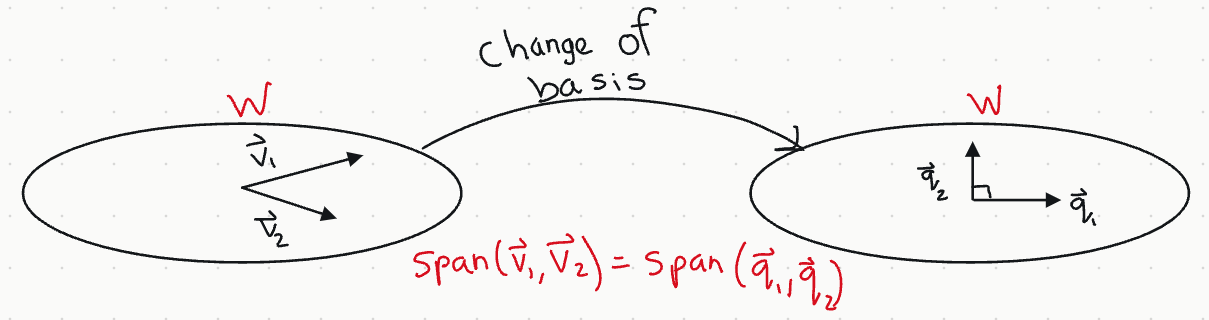
\includegraphics[width=0.8\textwidth]{change-to-ortho-basis}
		\caption{Change from linearly independent basis $\mathbf{v}_1,\mathbf{v}_2$
		to orthogonal basis $\mathbf{q}_1,\mathbf{q}_2$ without changing the subspace}
		\label{fig:change-to-ortho-basis}
	\end{figure}
	Equation~\ref{eqn:qr-factorization} is known as the \textbf{QR factorization of $X$}.
	Here, $Q$ is an orthonormal matrix such that $co\ell[Q] = co\ell[X]$, and $R$ is
	a full rank matrix. To obtain $Q$, we can use the \textbf{Gram-Schmidt Orthogonalization procedure}.
	The high-level steps are as follows:
	\begin{enumerate}[label=(\roman*)]
		\item Find an orthogonal set of basis vectors $\mathbf{v}_0,\mathbf{v}_1,\ldots,\mathbf{v}_p$.
		\item Normalize the vectors in the orthogonal set by dividing by their lengths:
		\begin{align*}
			\mathbf{q}_0=\frac{\mathbf{v}_0}{\|\mathbf{v}_0\|},\quad
			\mathbf{q}_1=\frac{\mathbf{v}_1}{\|\mathbf{v}_1\|},\quad
			\cdots\quad
			\mathbf{q}_p=\frac{\mathbf{v}_p}{\|\mathbf{v}_p\|}
		\end{align*}
		\item Tabulate the entries of $R$.
	\end{enumerate}
	The crucial step is the first one, which we explain in detail. Suppose the columns of
	$X$ are denoted $\mathbf{x}_{\cdot, 0},\mathbf{x}_{\cdot, 1},\ldots,\mathbf{x}_{\cdot, p}$.
	\begin{enumerate}[label=(\roman*)]
		\item We compute the orthogonal set in $p+1$ steps.
		\begin{itemize}
			\item  In step $0$, set
			$\mathbf{v}_{0}=\mathbf{x}_{\cdot, 0}$.
			\item In step $1$, set
			\begin{align*}
				\mathbf{v}_1=\mathbf{x}_{\cdot, 1}
				-\underset{\text{span}(\mathbf{v}_{0})}{\text{proj}(\mathbf{x}_{\cdot,1})}
			\end{align*}
			By removing the component of $\mathbf{x}_{\cdot, 1}$ in the direction of $\mathbf{v}_0$,
			we accomplish the goal of making $\mathbf{v}_0$ and $\mathbf{v}_1$ orthogonal
			(see Figure~\ref{fig:vec-proj-1d}).
			\begin{figure}
				\centering
				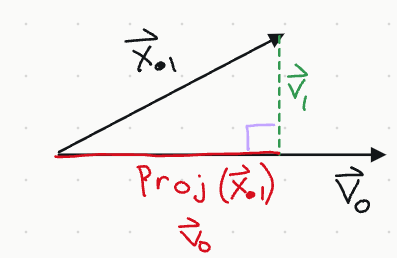
\includegraphics[width=0.4\textwidth]{vector-projection-1d}
				\caption{Removing the component of $\mathbf{x}_{\cdot, 1}$ in the
				direction of $\mathbf{v}_0$.}
				\label{fig:vec-proj-1d}
			\end{figure}
			\item In step $2$, set
			\begin{align*}
				\mathbf{v}_2=\mathbf{x}_{\cdot, 2}
				-\underset{\text{span}(\mathbf{v}_{0})}{\text{proj}(\mathbf{x}_{\cdot,2})}
				-\underset{\text{span}(\mathbf{v}_{1})}{\text{proj}(\mathbf{x}_{\cdot,2})}
			\end{align*}
			\item In general, for step $k$, where $1\leq k\leq p$, we have
			\begin{align*}
				\mathbf{v}_k=\mathbf{x}_{\cdot, k}
				-\sum_{j=0}^{k-1}\underset{\text{span}(\mathbf{v}_{j})}{\text{proj}(\mathbf{x}_{\cdot,k})}
			\end{align*}
		\end{itemize}
		\item Now we simply normalize $\mathbf{v}_k$ for $0\leq k\leq p$:
		\begin{align*}
			\mathbf{q}_k=\frac{\mathbf{v}_k}{\|\mathbf{v}_k\|}
		\end{align*}
		\item We will discuss this last step next time.
	\end{enumerate}
	
	\pagebreak
	\printbibliography
\end{document}